\documentclass[fleqn]{VRIH2025}
\setlength{\mathindent}{0cm}
\def\dl{\displaystyle}
\thispagestyle{empty}
\usepackage{bm}
\usepackage{multirow}
\usepackage{braket}
\usepackage{algorithm}
\pdfstringdefDisableCommands{\renewcommand*{\bm}[1]{#1}}

\begin{document}

\ensubject{Theoretical Physics}
\qyluntan
%Letter to the Editor??Article%??????
\ArticleType{Article}%??Article
%\SpecialTopic{Special Topic: New Challenges and New Physics in Future Cosmology}%???????
\Year{2025}
\Month{August}
\Vol{68}
\No{8}
\DOI{10.1007/s11433-025-2682-1}
\ReceiveDate{27 January 2025}
\RevisedDate{28 February 2025}
\AcceptDate{28 April 2025}
%\OnlineDate{27 June 2025}
%%%%%%%%%%%%%%%%%%%%%%%%%%%%%%%%%%%%%%%%%%%%%%%%%%%%%%%

%%% title: ????
%%%   \title{title}{title for citation}

\title{Advanced driver assistance system (ADAS) and machine learning (ML): The dynamic duo revolutionizing the automotive industry}{Advanced driver assistance system (ADAS) and machine learning (ML): The dynamic duo revolutionizing the automotive industry}

\author[1]{Shengqing GAO}{}
\author[2]{Qing GAO}{{gaoqing1024@swu.edu.cn}}
\author[3,1]{Yungui GONG}{}
\author[1]{Xuchen LU}{}


\AuthorCitation{Shengqing GAO, Qing GAO, Yungui GONG, Xuchen LU}

\address[1]{School of Physics, Huazhong University of Science and Technology,  Wuhan 430074, China}
\address[2]{School of Physical Science and Technology, Southwest University, Chongqing 400715, China}
\address[3]{Institute of Fundamental Physics and Quantum Technology, Department of Physics, School of Physical Science and Technology,\\
Ningbo University, Ningbo 315211, China}

\abstract{This work aims to build a comprehensive and effective fire emergency management system based on the Internet of Things (IoT) and achieve an actual intelligent fire rescue. A smart fire protection information system was designed based on the IoT. A detailed analysis was conducted on the problem of rescue vehicle scheduling and the evacuation of trapped persons in the process of fire rescue. Methods The intelligent fire visualization platform based on the three-dimensional (3D) Geographic Information Science (GIS) covers project overview, equipment status, equipment classification, equipment alarm information, alarm classification, alarm statistics, equipment account information, and other modules. The live video accessed through the visual interface can clearly identify the stage of the fire, which facilitates the arrangement of rescue equipment and personnel. The vehicle scheduling model in the system primarily used two objective functions to solve the Pareto Non-Dominated Solution Set Optimization: emergency rescue time and the number of vehicles. In addition, an evacuation path optimization method based on the Improved Ant Colony (IAC) algorithm was designed to realize the dynamic optimization of building fire evacuation paths. Results The experimental results indicate that all the values of detection signals were significantly larger in the smoldering fire scene at t=17s than the initial value. In addition, the probability of smoldering fire and the probability of open fire were relatively large according to the probability function of the corresponding fire situation, demonstrating that this model could detect fire. Conclusions The IAC algorithm reported here avoided the passages near the fire and spreading areas as much as possible and took the safety of the trapped persons as the premise when planning the evacuation route. Therefore, the IoT-based fire information system has important value for ensuring fire safety and carrying out emergency rescue and is worthy of popularization and application.
}

\keywords{Smart fire protection information system; Internet of things; Rescue vehicle scheduling; Optimal evacuation routes}

\maketitle


\section{Introduction}
%\subsection{Motivation}
The SFP came into being in the context of FP needs in the new era. SFP is an 
integral part of SC construction, mainly reflected in four aspects: smart 
prevention and control, smart management, smart operations, and smart 
command \cite{1}. Its application field covers all scenarios requiring FPC, 
such as public buildings, commercial buildings, real estate communities, and 
entertainment venues, especially in production enterprises with high risks, 
including factories of petroleum, chemical, flammable, and explosive 
materials. Entering the BD era, the continuous development of the computer 
technology revolution has significantly impacted the operation mode of each 
industry and provided technical support for the innovation of FP 
business \cite{2}. Menon and Vishnu-Menon \cite{3} pointed out that the 
intelligent FM system applies high-end technologies such as GIS, Wireless 
Communication Technology, Global Positioning System (GPS), and IoT terminals 
to the management, supervision, collection, and monitoring services of FP. 
These functions are reflected as the platform presentation in FM work, such 
as real-time updates and dynamic monitoring of various data, closed-loop 
management of inspection operation and maintenance work, and online display 
of personnel work conditions. The system integrates all elements and links 
in FP, breaks the barriers of information transmission, combines matches, 
and optimizes the online monitoring data and FP content, making the process 
of each link of FP management clearer. Alqourabah et al. implemented an 
intelligent fire detection system to detect fires using integrated sensors 
and alert homeowners and local fire departments to protect lives and 
assets \cite{4}. This system collects signals from different integrated 
detectors to forecast the probability of a fire and broadcast the prediction 
to all parties using the Global System for Mobile Communication 
modulator-demodulator associated with the system.


\section{Related work}

\subsection{Small form-factor pluggable information system}
\label{subsec:mylabel1}

The SFP came into being in the context of FP needs in the new era. SFP is an 
integral part of SC construction, mainly reflected in four aspects: smart 
prevention and control, smart management, smart operations, and smart 
command \cite{5} Its application field covers all scenarios requiring FPC, 
such as public buildings, commercial buildings, real estate communities, and 
entertainment venues Table~\ref{table PRA}, especially in production enterprises with high risks, 
including factories of petroleum, chemical, flammable, and explosive 
materials. Entering the BD era, the continuous development of the computer 
technology revolution has significantly impacted the operation mode of each 
industry and provided technical support for the innovation of FP 
business \cite{6}. Menon and Vishnu-Menon \cite{7} pointed out that the 
intelligent FM system applies high-end technologies such as GIS, Wireless 
Communication Technology, Global Positioning System (GPS), and IoT terminals 
to the management, supervision, collection, and monitoring services of FP. 
These functions are reflected as the platform presentation in FM work, such 
as real-time updates and dynamic monitoring of various data, closed-loop 
management of inspection operation and maintenance work, and online display 
of personnel work conditions. The system integrates all elements and links 
in FP, breaks the barriers of information transmission, combines matches, 
and optimizes the online monitoring data and FP content, making the process 
of each link of FP management clearer. Alqourabah et al. implemented an 
intelligent fire detection system to detect fires using integrated sensors 
and alert homeowners and local fire departments to protect lives and 
assets \cite{8}. This system collects signals from different integrated 
detectors to forecast the probability of a fire and broadcast the prediction 
to all parties using the Global System for Mobile Communication 
modulator-demodulator associated with the system.




\subsection{Emergency rescue}
EM is a system process problem, including information collection, 
transportation, emergency response, and material distribution. Wang et al. 
put forward the idea of active disaster relief in response to the ER of 
sudden fires, that is, the coordinated, centralized control of ventilation, 
air exhaust, smoke blocking, smoke exhausting, and other facilities to 
assist passengers in evacuation and firefighting \cite{9}. The authors 
analyzed complex subways' ventilation and smoke exhaust methods at 
multi-layer intersections, selected a typical transfer station, and 
established a numerical model. Besides, the combined control of fire smoke 
was analyzed using six ventilation modes, and several numerical simulations 
were carried out using the fire dynamics simulator software. Then, according 
to the characteristics of different fire sources and smoke control 
scenarios, a multi-element information fusion RM model was established, such 
as ventilation paths, fan characteristics, smoke exhaust channels, and smoke 
blocking facilities. The author finally proved that the ER platform is 
conducive to efficient fire rescue and the safe escape of personnel in 
emergencies. Tang et al. established a timely and effective Satellite Remote 
Sensing Emergency Monitoring Information Service (SRSEMIS) framework as a 
vital part of the natural disaster ER \cite{10}. It focuses on key 
technologies such as comprehensive data management, multi-source data 
processing, disaster response information analysis, and rapid release of 
information services. Meanwhile, the SRSEMIS framework realized the 
real-time transmission of disaster data before and after the disaster 
through the specific application in the emergency remote sensing monitoring 
of the 3.30 Forest fire in Muli County, Sichuan. In the ER process, it is 
imperative to release remote sensing interpretation images of disaster areas 
promptly and improve comprehensive information services such as 3D terrain 
characterization, rescue accessibility prediction, and fire change analysis.
\begin{equation}
\label{eq:D_M}
    D_{M}(z)=\frac{1}{H_0 \sqrt{|\Omega_{k0}|}} \text{sinn} \left[\sqrt{|\Omega_{k0}|} \int_0^z \frac{\textrm{d} x}{E(x)}\right],
\end{equation}
where $H_0=H(z=0)$ is the Hubble constant, $E(z)=H(z)/H_0$ is the dimensionless Hubble parameter,
and $\text{sinn}(\sqrt{|\Omega_{k0}|}x)/\sqrt{|\Omega_{k0}|}=\sinh(\sqrt{|\Omega_{k0}|}x)/\sqrt{|\Omega_{k0}|}$, $x$
and $\sin(\sqrt{|\Omega_{k0}|}x)/\sqrt{|\Omega_{k0}|}$ for $\Omega_{k0}>0$,
$\Omega_{k0}=0$ and $\Omega_{k0}<0$, respectively.
For a spatially flat universe, $\Omega_{k0}=0$,
\begin{equation}
\label{eq:D_M_flat}
D_M(z)=\frac{1}{H_0}\int_{0}^{z}\frac{\textrm{d} x}{E(x)}.
\end{equation}

\subsection{Intelligent fire evacuation path}

When a fire occurs, the intelligent fire evacuation system implements fire 
evacuation guidance in the form of optical ground flow according to the fire 
alarm information of the fire alarm system and the direction of the spread 
of smoke. It can accurately give Evacuation Paths (EPs) instructions, help 
people in the building choose the escape route, guide the safe escape 
direction, and ensure the personal safety of the masses \cite{11}. After a 
fire, an AI application can guide occupants to secure evacuation routes 
while helping rescuers enter the building. Gomaa et al. proposed an 
integrated trained AI and sensor-based data collection system for the 
short-term prediction of fire occurrence behavior, structural integrity, and 
optimal escape paths. It can also issue escape instructions to users via 
mobile devices or public address systems \cite{12}. Cao et al. proposed an 
intelligent EP optimization scheme for dense crowds in buildings \cite{13}. 
First, they used an artificial Fish Swarm Algorithm-based agglomeration 
model without the help of an instructor. Second, a single-layer evacuation 
model based on the improved K-Nearest Neighbors algorithm was used to 
classify individuals. This model could help individuals choose the nearest 
stairs, saving escape time.

Existing studies have systematically discussed the design of SFP systems and 
the application of critical technologies. This work built an SFP information 
system based on visualization technology and combined it with IoT technology 
to achieve high application value in FMDM. In addition, in-depth research 
was carried out on the most critical RV scheduling and personnel escape path 
optimization in the SFP information system.


\begin{figure}[!tb]
\centering
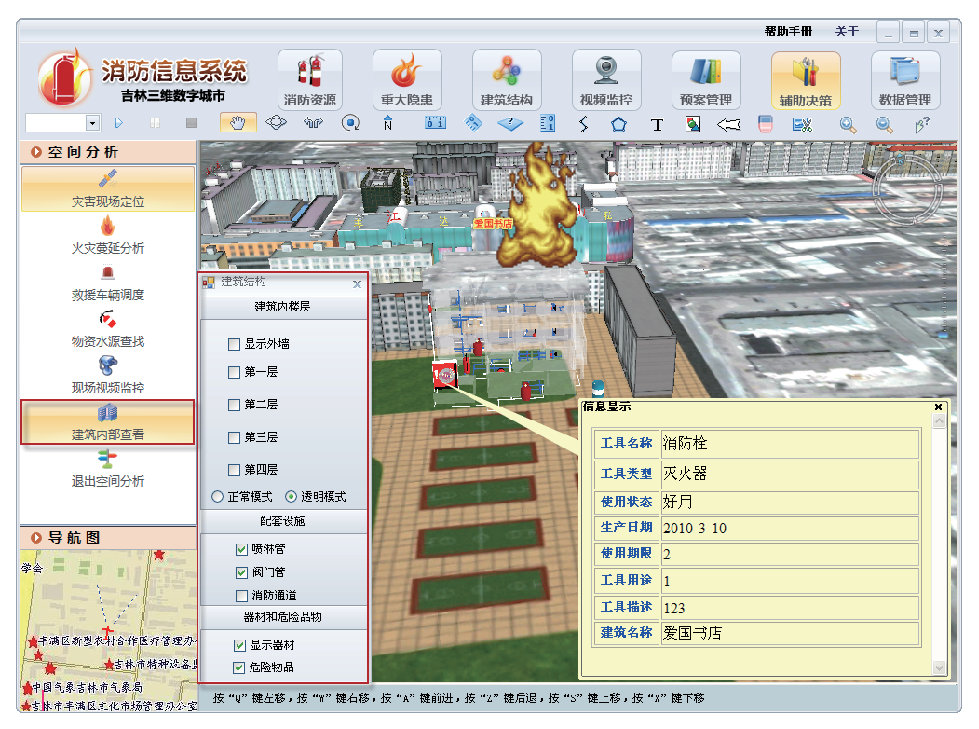
\includegraphics{VRIH-t1.eps}
   \caption{The architecture of the IFFV platform.}
    \label{fig:structure}
\end{figure}


\section{Traffic information processing and task scheduling in digital twins 
scenarios}

\subsection{Smart fire visualization information platform based on the 
three-dimensional geographic information science}

At present, the main problem with fire rescue is that the arrangement of 
rescue resources is not systematic enough. Most SFP systems in operation or 
under research are developed based on two-dimensional (2D) geographic 
information systems. The 2D geographic information system can only display 
the plane information of buildings and structures but cannot display the 3D 
geographic data. The new large-scale and low-cost 3D modeling technology is 
gradually maturing \cite{14}, which has significant practical value for the 
critical units of FP, FM, information entry, firefighting plan, and on-site 
command of key monitoring areas of FP \cite{15}. The 3D trend for the SFP 
platform has become unstoppable. Therefore, it is imminent to design and 
implement a high-load, high-integration SFP information platform based on 3D 
GIS. Figure \ref{fig:structure} shows the architecture of the IFFV platform designed here. 
After successfully logging in to the platform, users will see the main 
content displayed on the home page, including project overview, device 
status, device classification, device alarm information, alarm 
classification, alarm statistics, and device account information. Users can 
select the map as a Building Information Modeling model to display warnings 
from any sensors. Hidden hazard management includes hazard inspection, 
hazard treatment, and hazard records. The purpose of hidden danger 
inspection is to enable the system to distribute work orders to engineering 
personnel after an alarm or a hidden danger occurs. After processing, 
engineers fill in relevant work order task records in the system for the 
historical query. 




\InterestConflict{The authors declare that they have no conflict of interest.}

\AuthorContributions{\textbf{Harsh Shah:} Conceptualization, Writing�Coriginal draft. \textbf{Karan Shah:} Writing�Creview \& editing. \textbf{Kushagra Darji:} Data curation, Methodology. \textbf{Adit Shah:} Validation. \textbf{Manan Shah:} Conceptualization, Supervision.}



\begin{thebibliography}{100}

\bibitem{1}Mu X W, Zhou X, Wang W, Xiao Y L, Liao C, Han L F, Kan Y C, Song L. Design of compressible flame retardant grafted porous organic polymer based separator with high fire safety and good electrochemical properties. Chemical Engineering Journal, 2021, 405, 126946\\
\url{DOI: 10.1016/j.cej.2020.126946}


\bibitem{2}Li L, Shao X M, Zhao Z, Liu X L, Jiang L C, Huang K, Zhao S. Synergistic fire hazard effect of a multifunctional flame retardant in building insulation expandable polystyrene through a simple surface-coating method. ACS Omega, 2020, 5(1): 799�C807\\
\url{DOI: 10.1021/acsomega.9b03541}


\bibitem{3} Xu W Z, Yan H Y, Wang G S, Qin Z Q, Fan L J, Yang Y X. A silica-coated metal-organic framework/graphite-carbon nitride hybrid for improved fire safety of epoxy resins. Materials Chemistry and Physics, 2021, 258, 123810\\
\url{DOI: 10.1016/j.matchemphys.2020.123810}


\bibitem{4} Zhang G W, Yan S, Zhu G Q, Feng P Y, Jia B Y. Smart firefighting construction in China: status, problems, and reflections. Fire and Materials, 2020, 44(7): 479�C486\\
\url{DOI: 10.1002/fam.2800}


\bibitem{5} Ning H S, Li Y F, Shi F F, Yang L T. Heterogeneous edge computing open platforms and tools for Internet of Things. Future Generation Computer Systems, 2020, 106: 67�C76\\
 \url{DOI: 10.1016/j.future.2019.12.036}

\bibitem{6} Meena S R, Albrecht F, H?lbling D, Ghorbanzadeh O, Blaschke T. Nepalese landslide information system (NELIS): a conceptual framework for a web-based geographical information system for enhanced landslide risk management in Nepal. Natural Hazards and Earth System Sciences, 2021, 21(1): 301�C316\\
    \url{DOI: 10.5194/nhess-21-301-2021}

\bibitem{7} Sungheetha D A, Sharma R D R. Real time monitoring and fire detection using internet of things and cloud based Drones. Journal of Soft Computing Paradigm, 2020, 2(3): 168�C174\\
\url{DOI: 10.36548/jscp.2020.3.004}


\bibitem{8} Yahyaoui A, Abdellatif T, Yangui S M, Attia R. READ-IoT: reliable event and anomaly detection framework for the Internet of Things. IEEE Access, 9: 24168--24186\\
\url{DOI: 10.1109/access.2021.3056149}


\bibitem{9} Badshah A, Ghani A, Ahsan Qureshi M, Shamshirband S. Smart security framework for educational institutions using Internet of Things (IoT). Computers, Materials \& Continua, 2019, 61(1): 81�C101\\
\url{DOI: 10.32604/cmc.2019.06288}


\bibitem{10}  Jo B W, Khan R M A, Javaid O. Arduino-based intelligent gases monitoring and information sharing Internet-of-Things system for underground coal mines. Journal of Ambient Intelligence and Smart Environments, 2019, 11(2): 183�C194\\    
\url{DOI: 10.3233/ais-190518}

\bibitem{11} Naresh V S, Pericherla S S, Sita Rama Murty P, Reddi S. Internet of 
Things in healthcare: architecture, applications, challenges, and solutions. 
Computer Systems Science and Engineering, 2020, 35(6): 411�C421\\
\url{DOI: 10.32604/csse.2020.35.411}

\bibitem{12} Wu X Q, Park Y, Li A, Huang X Y, Xiao F, Usmani A. Smart detection of 
fire source in tunnel based on the numerical database and artificial 
intelligence. Fire Technology, 2021, 57(2): 657�C682\\
\url{DOI: 10.1007/s10694-020-00985-z}

\bibitem{13} Beg A, Qureshi A R, Sheltami T, Yasar A. UAV-enabled intelligent traffic 
policing and emergency response handling system for the smart city. Personal 
and Ubiquitous Computing, 2021, 25(1): 33�C50\\
\url{DOI: 10.1007/s00779-019-01297-y}

\bibitem{14} Eini R, Linkous L, Zohrabi N, Abdelwahed S. Smart building management 
system: Performance specifications and design requirements. Journal of 
Building Engineering, 2021, 39: 102222\\
\url{DOI: 10.1016/j.jobe.2021.102222}

\bibitem{15} Zhang Y C, Geng P P, Sivaparthipan C B, Muthu B A. Big data and 
artificial intelligence based early risk warning system of fire hazard for 
smart cities. Sustainable Energy Technologies and Assessments, 2021, 45, 
100986\\
\url{DOI: 10.1016/j.seta.2020.100986}

\end{thebibliography}

\end{document}
